\documentclass[12pt]{article}
\parindent=0.25in

\setlength{\oddsidemargin}{0pt}
\setlength{\textwidth}{440pt}
\setlength{\topmargin}{0in}
\usepackage{amssymb}
\usepackage{amsfonts}
\usepackage{amsmath}
\usepackage{cancel}
\usepackage{latexsym}
\usepackage[center]{subfigure}
\usepackage{epsfig}
\usepackage{3952}
\usepackage{3952-thm}
\usepackage{pstricks,pst-node,pst-tree}
\usepackage{soul, xcolor}
\usepackage{bbold}
\usepackage[backref, colorlinks,citecolor=blue,bookmarks=true]{hyperref}  


% \def\size{\mathop{\rm{size}}\nolimits}
% \def\depth{\mathop{\rm{depth}}\nolimits}
% \newtheorem{theorem}{Theorem}
% \newtheorem{lemma}{Lemma}
% \newtheorem{corollary}{Corollary}
% \newtheorem{fact}{Fact}
% \newtheorem{definition}{Definition}
% \newtheorem{claim}{Claim}
% \newenvironment{proof}{\noindent \textbf{Proof:}}{$\Box$}
% \newenvironment{proofsketch}{\noindent \textbf{Proof Sketch:}}
% \newcommand{\infint}{\int_{-\infty}^\infty}
% \newcommand{\intunit}{\int_{-1}^1}
% \newcommand{\binclass}{x \in \{0,1\}^n}
% \newcommand{\example}{\textbf{Example:} }
% \newcommand{\observation}{\textbf{Observation:} }
% \newcommand{\note}{\textbf{Note:} }
% \newcommand{\noisy}[1]{N_\epsilon(#1)}
% \newcommand{\noisens}[1]{ns_\epsilon(#1)}
% \newcommand{\eg}{{\it e.g.,\ }}
% \newcommand{\Inf}{{\mathrm{Inf}}}
% \newcommand{\PAR}{{\mathrm{PAR}}}
% \def\poly{\mathop{\rm{poly}}\nolimits}
% \def\eps{{\epsilon}}
% \newcommand{\E}{{\bf E}}
% \def\through{{,\ldots,}}


\pagestyle{headings}    % Go for customized headings

\newcommand{\handout}[5]{
   \noindent
   \begin{center}
   \framebox{
      \vbox{
    \parbox[t]{4in} {\bf #1 } \vspace{3mm}  {\hfill \bf #2 }
       \vspace{2mm}
       \hbox to 6.00in { {\Large \hfill #5  \hfill} }
       \vspace{1mm}
       \hbox to 6.00in { {\it #3 \hfill #4} }
      }
   }
   \end{center}
   \vspace*{1mm}
}

\hypersetup{linkcolor=magenta}

\begin{document}

\handout{MATH 3952 (Undergraduate Seminar): Quantum Information Theory}{Spring 2024}
{Organizer: Patrick Lei; Presenter: Nathan Raghavan}
{Scribe: Mark Chen}{Lecture 2, Talk 1: February 5, 2024}

\thispagestyle{plain}
% \setcounter{section}{-1}
\section*{Chapter 2: Qubits}
\section{Composing Quantum Operations}
Even though a single classic bit $0/1$ has nothing too interesting to it, a single qubit interference sets up the fundamental properties that help build up to a full QC. So, we look at it more carefully.

Notice that for a single qubit, there are only four possible things that a program can do to it, namely the following paths from one type of a single qubit input to one type of of a single qubit next step:
\begin{center}
    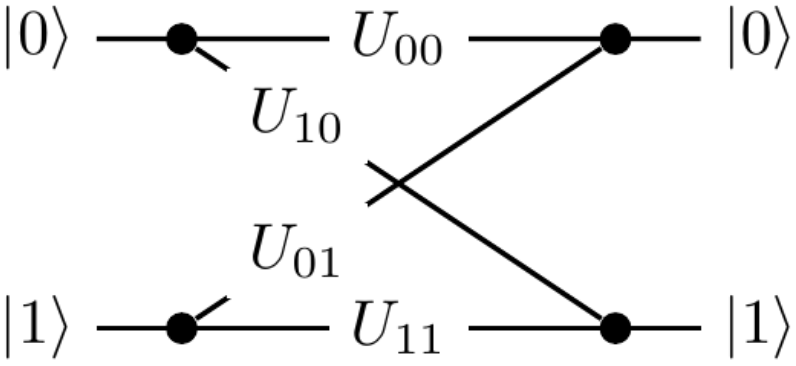
\includegraphics[width = 15em]{images/1.jpg}
\end{center}
, where the $$
U = \begin{bmatrix}
U_{00} & U_{01}\\
U_{10} & U_{11}
\end{bmatrix}
$$ is defined the way that we have seen before (as a reminder, $U_{01}$ means to end in state $0$ from an initial state of $1$).

So, these can keep going for any arbitrary number of times, with the output of this step being the input to the next step. So, now, suppose we have two computational steps, $U$ and $V$, instead, then we have something like the illustrated below:
\begin{center}
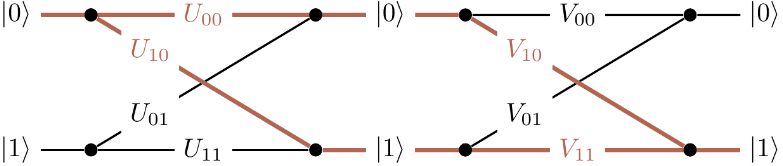
\includegraphics[width = 25em]{images/2.jpg}
\end{center}
, then it is clearly the case that $$
\Ket{k} \mapsto \underset{l}{\sum}U_{lk}\Ket{l} \mapsto  \underset{l}{\sum}U_{lk}\prt{\underset{m}{\sum}V_{ml}\Ket{m}}
$$. We can simplify this as: $$
\Ket{k} \mapsto  \underset{l}{\sum}U_{lk}\prt{\underset{m}{\sum}V_{ml}\Ket{m}} = \underset{l}{\sum}\underset{m}{\sum}V_{ml}U_{lk}\Ket{m} = \underset{m}{\sum}(VU)_{mk}\Ket{m}
$$

\begin{intuition}
Especially pay attention to the last step: $$
\underset{m}{\sum}(VU)_{mk}\Ket{m}
$$. This gives the amplitude that input $\Ket{k}$ evolves to $\Ket{m}$ via a specific intermediate state $\Ket{l}$ is given by $V_{ml}U_{lk}$, and then we sum over all possible values of $L$.

In essence, the matrix multiplication, $VU$ (notice that the order is from right to left in the order that operations are taken), takes care of both of the multiplication and addition needed of amplitudes corresponding to different computational paths.
\end{intuition}

\begin{definition}[Qubit]
The two-state machine that was described above is usually realized as a controled evolution of a two-state system, called a quantum bit, or qubit for short; $\eg$ $\Ket{0}$ may be the \textbf{ground stat}e, $\Ket{1}$ may be the \textbf{excited state}, and pulses of light of appropriate \underline{frequency, duration and intensity} can:
\begin{itemize}
    \item take the atom back and forth between the basis states (by implementing the logical $\NOT$ gate).
    \item transition the state to somewhere in between that have no classical analogue. Those can generally be described by $$
    \Ket{\psi} = a_0\Ket{0} + a_1\Ket{1}
    $$ for some $a_0, a_1\in \CC$ and $|a_0|^2 + |a_1|^2 = 1$.
    
    Any such physically admissible operatioin $U$ on a qubit can be described by a $2\times 2$ matrix $U$: $$
    \begin{bmatrix}
    a_0'\\
    a_1'
    \end{bmatrix} = \begin{bmatrix}
    U_{00} & U_{01}\\
    U_{10} & U_{11}
    \end{bmatrix}\begin{bmatrix}
    a_0\\
    a_1
    \end{bmatrix}
    $$ which is just a specific form of the general form we derived before in this subsection.
\end{itemize}
\end{definition}

\section{Quantum Gates and Circuits}
\begin{definition}[Quantum (Logic) Gate]
A quantum (logic) gate is a device that performs a \underline{fixed unitary operation} on \underline{selected qubits} in a \underline{fixed period of time}.
\end{definition}

\begin{definition}[Quantum Circuits]
A quantum circuit is a device consisting of \underline{quantum} \underline{logic gates} whose computational steps are \underline{synchronized in time}.
\begin{center}
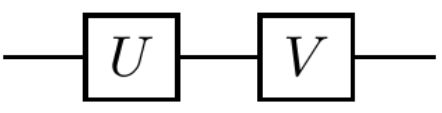
\includegraphics[width = 12em]{images/3.jpg}
\end{center}
is an example of a seequence of two gates, each of which can be represented by a unitary matrix, or $VU$ as a whole.
\end{definition}

\begin{definition}[Size $\&$ Depth]
The \textbf{size} of a circuit is the number of quantum logic gates, and the \textbf{depth} is, as the gates in a circuit can be divided into layers (gates within each layer can be seen as happening at the same time), the number of such layers.
\end{definition}

\begin{proposition}[Circuit with more qubits as input]
Notice that, no matter how many gates we have for a single qubit, say $A$, $B$ and $C$ in this order, we can represent the whole circuit as a single unitary matrix: $$
U = CBA\text{, where } UU^\dag = \mathbb{1}
$$, which means any circuit for one single qubibt is a member of $U(2)$.

This result can be generalized: any $n$-qubit input circuit can be represented by a member of $$\boxed{U(2^n)}$$. Here is an example for why:
\begin{center}
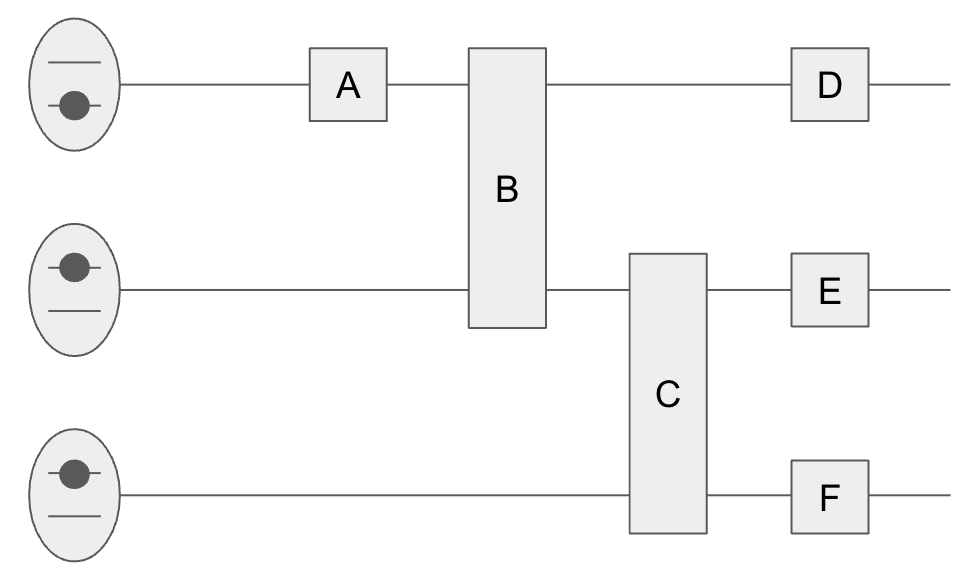
\includegraphics[width = 20em]{images/4.jpg}
\end{center}
Though it is hard to directly multiply each matrix that represent each of the gates just like for the case of a single qubit, it is not hard to understand why a $U(2^n)$ element would suffice. For example, $B$ can be represented by a $2\times 2$ matrix, because it takes $2^2$ inputs and produce $2^2$ outputs. That is, in general, a $2^3$ matrix is sufficient to represent anything that is physically admissible for a $3$-qubit circuit. Thus, we can generalize this to $U(2^n)$ for any $n$-qubit.
\end{proposition}

\section{Single Qubit Interference}
We have defined and discussed Hadamard gates and phase-shift gates already. Recall that, up to many equivalent forms, $$
\begin{aligned}
H
    &= \frac{1}{\sqrt{2}}\begin{bmatrix}
    1 & 1\\
    1 & -1
    \end{bmatrix}\\
P_\varphi
    &= \begin{bmatrix}
        1 & 0\\
        0 & e^{i\varphi}
    \end{bmatrix}
\end{aligned}
$$. Sometiems we denote $H$ going with specific qubit input as:$$
\begin{aligned}
\Ket{+} &:= H\Ket{0} = \frac{1}{\sqrt{2}}\prt{\Ket{0} + \Ket{1}}\\
\Ket{-} &:= H\Ket{1} = \frac{1}{\sqrt{2}}\prt{\Ket{0} - \Ket{1}}
\end{aligned}
$$

Recall that we also already wrote this following before: $$
HP_\varphi H = \frac{1}{\sqrt{2}}\begin{bmatrix}
    1 & 1\\
    1 & -1
    \end{bmatrix}\begin{bmatrix}
        1 & 0\\
        0 & e^{i\varphi}
    \end{bmatrix}\frac{1}{\sqrt{2}}\begin{bmatrix}
    1 & 1\\
    1 & -1
    \end{bmatrix} = \frac{1}{2}e^{\frac{\varphi}{2}}\begin{bmatrix}
        \cos\frac{\varphi}{2} & -i\sin\frac{\varphi}{2}\\
        -i\sin\frac{\varphi}{2} & \cos\frac{\varphi}{2}
    \end{bmatrix}
$$, so applying this circuit on a single qubit gives us $$
HP_\varphi H \begin{bmatrix}
    \Ket{0}\\
    \Ket{1}
\end{bmatrix} = \frac{1}{2}e^{\frac{\varphi}{2}}\begin{bmatrix}
    \cos\frac{\varphi}{2} & -i\sin\frac{\varphi}{2}\\
    -i\sin\frac{\varphi}{2} & \cos\frac{\varphi}{2}
\end{bmatrix}\begin{bmatrix}
    \Ket{0}\\
    \Ket{1}
\end{bmatrix}
$$, which would give that $$
\Ket{0} \overset{HP_\varphi H}{\mapsto} \cos\frac{\varphi}{2}\Ket{0} - i\sin\frac{\varphi}{2}\Ket{1}
$$

\begin{remark}
The phase shift $\varphi$ is the only thing that we have parametrized that tweaks the final output, since the two Hadamard gates simply opens and closes the interference and won't be parametrizable.

This makes the above Hadamard-Phase-Shift-Hadamard cifcuit very common, because it is a natural progression of quantum computation where we 1. first prepare different computational paths, 2. we introduce phase shift into these different computational paths, and 3. we bring the computational paths together at the output.
\end{remark}

\begin{remark}
Finally, since $$\cos\frac{\varphi}{2}\Ket{0} - i\sin\frac{\varphi}{2}\Ket{1}$$ describes the probability amplitude of the superposition, it is easy to see by definition that:
\begin{itemize}
    \item $\Pr[0] = \cos^2 \frac{\varphi}{2}$
    \item $\Pr[1] = \sin^2 \frac{\varphi}{2}$
\end{itemize}
\end{remark}

\section{$\sqrt{\NOT}$}
What we want to do is to design a logic gate such that when two of this gate is applied to in a sequence, the output is always the negation of the input:
\begin{center}
    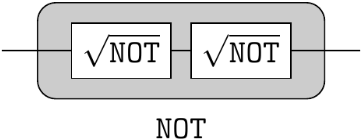
\includegraphics[width = 15em]{images/5.jpg}
\end{center}

\begin{definition}[$\sqrt{\NOT}$]
Recall from linear algebra that a logical $\NOT$ gate is the matrix: $$
\NOT = \begin{bmatrix}
0 & 1\\
1 & 0
\end{bmatrix}
$$, so what we want is to find a matrix such that it's square is $\NOT$. It can be verified that the following matrix would suffice: $$
\sqrt{\NOT} = \frac{1}{2}\begin{bmatrix}
1+i & 1-i\\
1-i & 1+i
\end{bmatrix} = \boxed{\frac{1}{\sqrt{2}}\begin{bmatrix}
e^{i\frac{\pi}{4}} & e^{-i\frac{\pi}{4}}\\
e^{-i\frac{\pi}{4}} & e^{i\frac{\pi}{4}}
\end{bmatrix}}
$$
\end{definition}

\begin{remark}
Since, now, the kind of operations like $\sqrt{\NOT}$ are justified by quantum theory, many logical operations are possible since they now have faithful physical models for them!
\end{remark}

\section{Phase Gates Galore}
\begin{remark}
Even though $$
P_\varphi = \begin{bmatrix}
1 & 0\\
0 & e^{i\varphi}
\end{bmatrix}
$$ is a form commonly used in the QIT community, $$
P_\varphi = \begin{bmatrix}
e^{-i\frac{\varphi}{2}} & 0\\
0 & e^{i\frac{\varphi}{2}}
\end{bmatrix}
$$ is a convenient and equivalent form (because equivalent up to global phase factor). The latter is useful because:
\begin{itemize}
    \item It has determinant $1$.
    \item It \hl{belongs to $SU(2)$}.
\end{itemize}
\end{remark}

\begin{definition}
There are a few specific and often-used $P_\varphi$ gates that merit their own names:
\begin{itemize}
    \item (Phase-flip) When $\varphi = \pi$, $e^{i\varphi} = -1$ (probably the most important out of these as it is one of the \textbf{Pauli operators}).
    \item ($\frac{\pi}{4}$-phase) When $\varphi =\frac{\pi}{2}$, $e^{i\varphi} = i$.
    \item ($\frac{\pi}{8}$-phase) When $\varphi =\frac{\pi}{4}$, $e^{i\varphi} = e^{i\frac{\pi}{4}}$.
\end{itemize}
The reason why $\frac{\pi}{4}$ and $\frac{\pi}{8}$ are not directly the value of $\varphi$ in our definition is because they are actually the phases in their corresponding versions in $SU(2)$.
\end{definition}

\begin{remark}
We will see soon how $SU(2)$ is related to $SO(2)$, how they describe $3$-D space (formally representation theory of Lie algebras).
\end{remark}



\end{document}